\documentclass[a4paper,10pt]{article}
\usepackage{graphicx}
\usepackage[utf8]{inputenc}
\usepackage[T1]{fontenc}
\usepackage{tgheros}
\usepackage{array}
\usepackage{xcolor}
\usepackage{amsmath}
\usepackage{sfmath}
\renewcommand{\familydefault}{\sfdefault}
\setlength{\oddsidemargin}{-5.4mm}
\setlength{\textwidth}{170mm}
\setlength{\topmargin}{-5.4mm}
\setlength{\headheight}{0mm}
\setlength{\headsep}{0mm}
\setlength{\textheight}{257mm}
\setlength{\footskip}{0mm}
\setlength{\parindent}{0pt}
\pagestyle{empty}
\begin{document}
% JMO Spectrum Library TM 30 report -- LaTeX include file
\newcommand{\Source}{some 4000K LED}
\newcommand{\Manufacturer}{unknown manufacturer}
\newcommand{\Date}{2024-04-18}
\newcommand{\Model}{unknown model}
\newcommand{\SpectrumGraphics}{SpectrumGraphics.eps}
\newcommand{\ChromaShiftGraphics}{ChromaShiftGraphics.eps}
\newcommand{\ColorVectorGraphics}{ColorVectorGraphics.eps}
\newcommand{\HueShiftGraphics}{HueShiftGraphics.eps}
\newcommand{\FidelityGraphics}{FidelityGraphics.eps}
\newcommand{\IndividualFidelityGraphics}{IndividualFidelityGraphics.eps}
\newcommand{\Notes}{results from TM30 test run}
\newcommand{\xVal}{0.3770}
\newcommand{\yVal}{0.3678}
\newcommand{\uprimeVal}{0.2264}
\newcommand{\vprimeVal}{0.4970}
\newcommand{\RaVal}{85}
\newcommand{\RnineVal}{28}
\newcommand{\RthirteenVal}{87}

{\Large
\begin{center}
\textbf{IES TM-30-18-Color Rendition Report}
\end{center}}

\makebox[15mm][l]{\textbf{Source:}}\colorbox{black!5}{\strut\makebox[63mm][l]{\Source}}%
\hspace{10mm}%
\makebox[25mm][l]{\textbf{Manufacturer:}}\colorbox{black!5}{\strut\makebox[53mm][l]{\Manufacturer}}

\makebox[15mm][l]{\textbf{Date:}}\colorbox{black!5}{\makebox[63mm][l]{\strut\Date}}%
\hspace{10mm}%
\makebox[15mm][l]{\textbf{Model:}}\colorbox{black!5}{\makebox[63mm][l]{\strut\Model}}

\begin{minipage}[b][128mm]{0.48\textwidth}
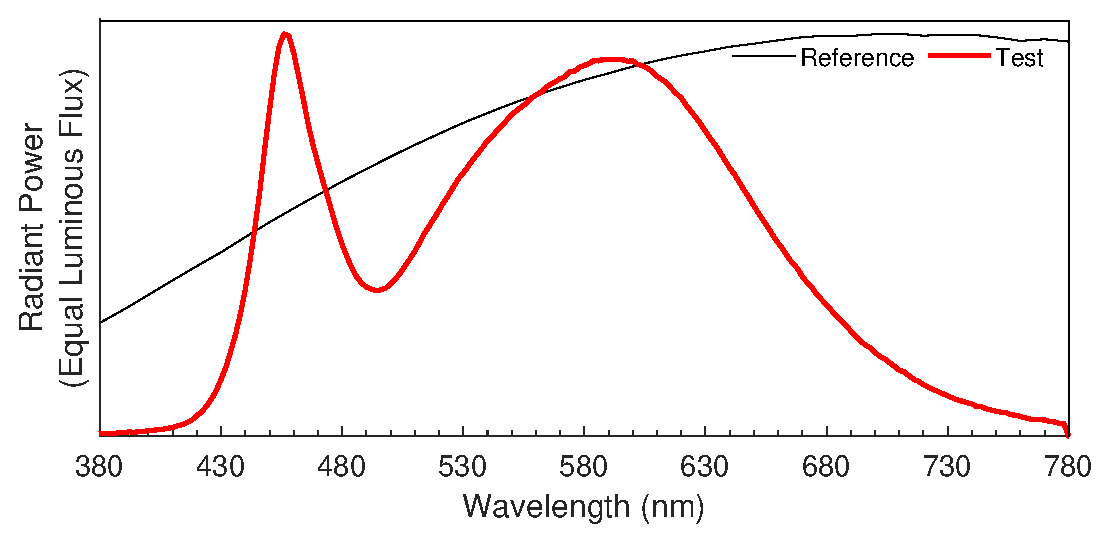
\includegraphics[width=\textwidth]{\SpectrumGraphics}\\[3mm]
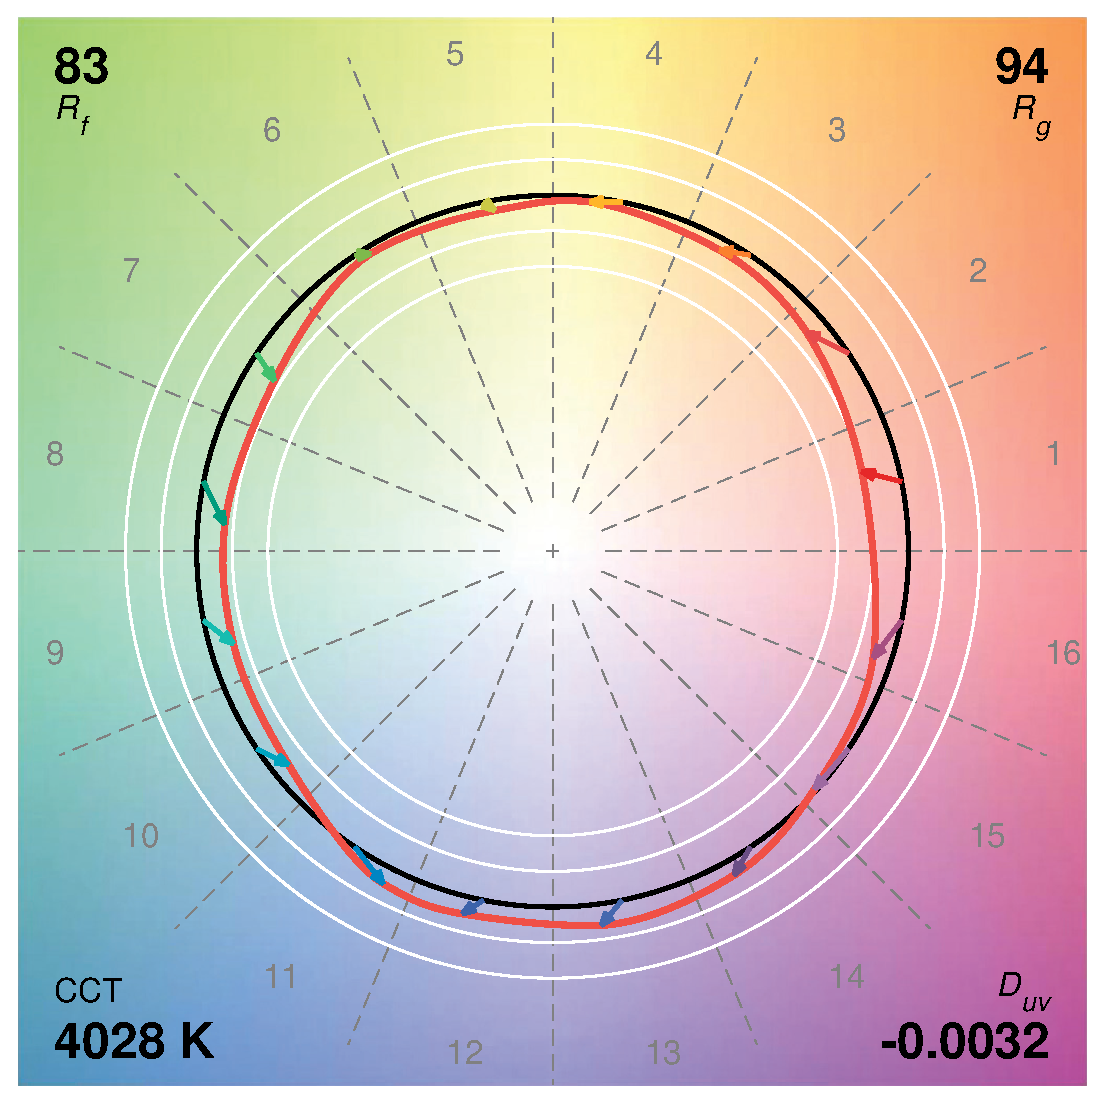
\includegraphics[width=\textwidth]{\ColorVectorGraphics}%
\end{minipage}%
\hspace{0.04\textwidth}%
\begin{minipage}[b][125mm]{0.48\textwidth}
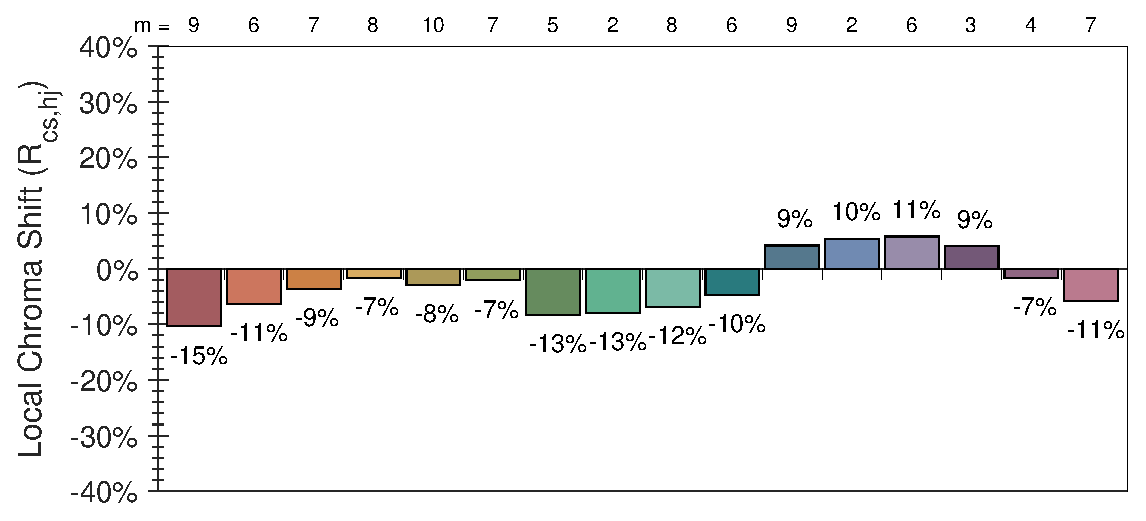
\includegraphics[width=\textwidth]{\ChromaShiftGraphics}
\par\vfill\par
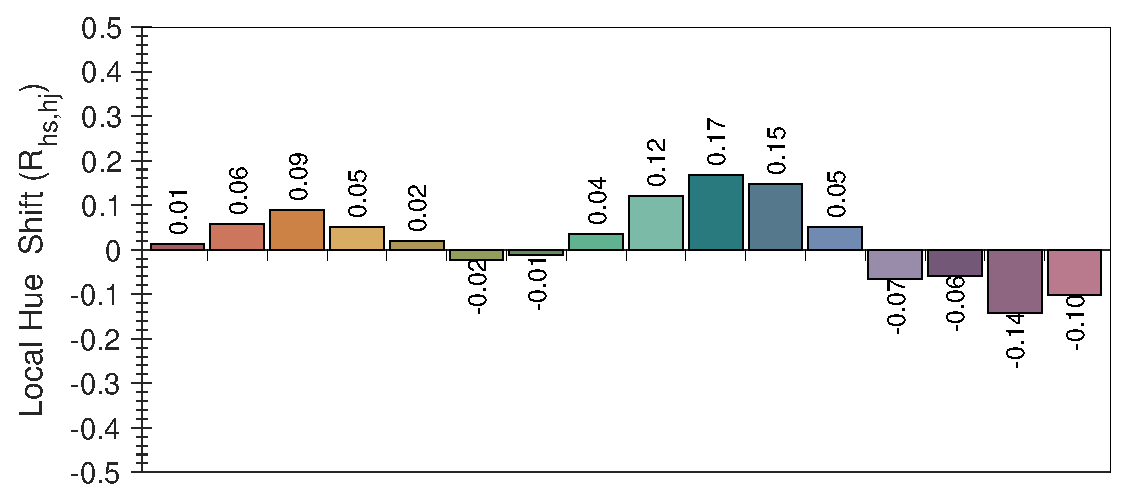
\includegraphics[width=\textwidth]{\HueShiftGraphics}
\par\vfill\par
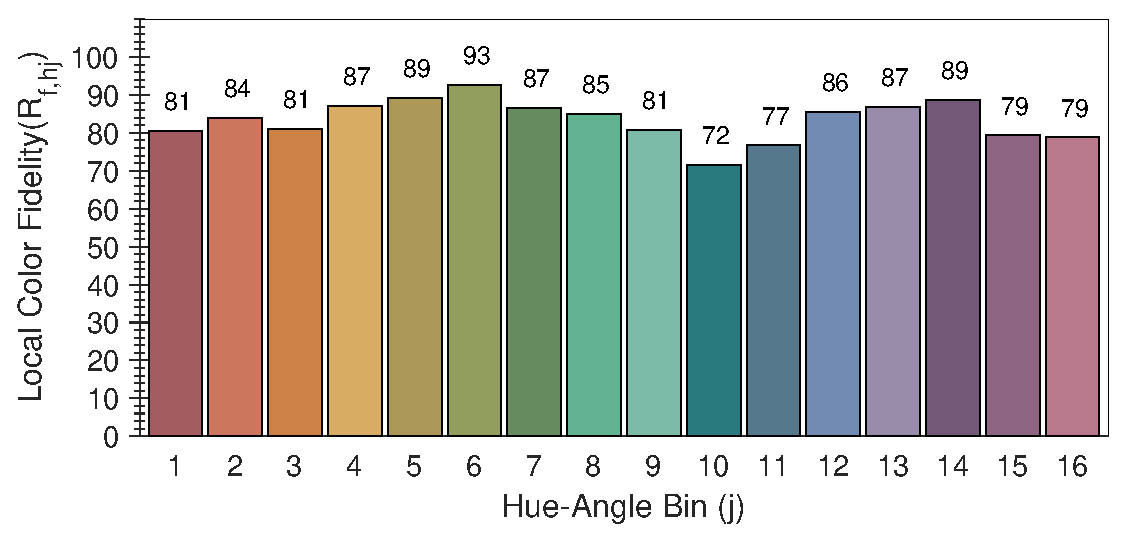
\includegraphics[width=\textwidth]{FidelityGraphics}
\end{minipage}

\vspace{3mm}
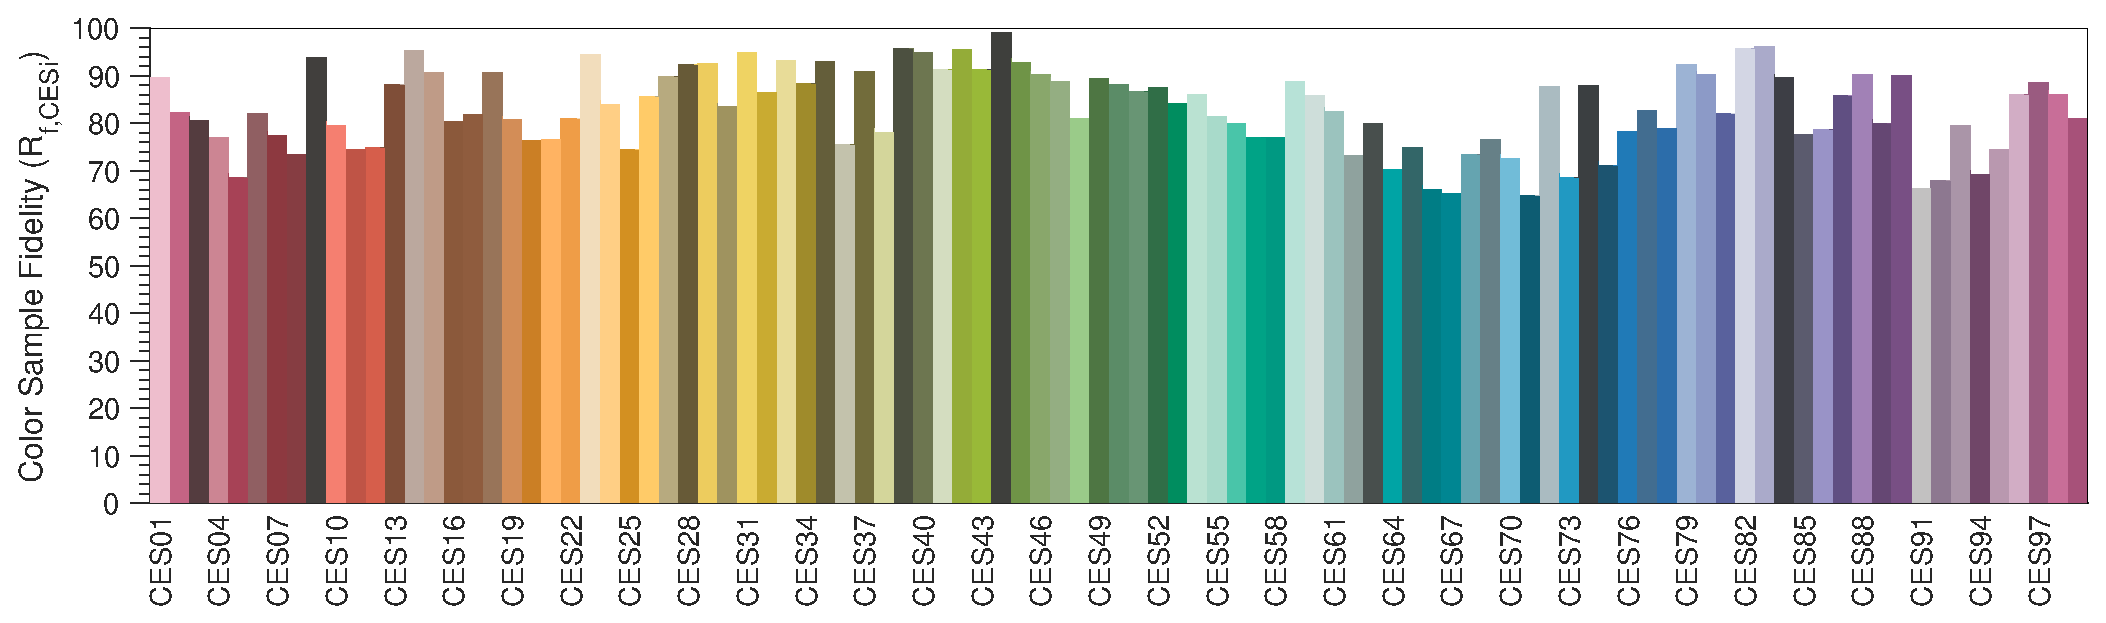
\includegraphics[width=\textwidth]{\IndividualFidelityGraphics}
\vspace{3mm}

\begin{minipage}[t][28mm]{90mm}
\makebox[15mm][l]{\textbf{Notes:}}\colorbox{black!5}{\strut\parbox[t][28mm]{73mm}{\Notes}}%
\end{minipage}
\hspace{5mm}
\raisebox{-12mm}{
\begin{tabular}{cl}
	\textit{x} & \xVal \\[2mm]
	\textit{y} & \yVal \\[2mm]
	\textit{u'} & \uprimeVal \\[2mm]
	\textit{v'} & \vprimeVal \\
\end{tabular}
}
\hspace{5mm}
\raisebox{-12mm}{
\framebox[40mm]{
\centering
\begin{tabular}{lr}
	\multicolumn{2}{c}{CIE 13.3-1995}\\
	\multicolumn{2}{c}{(CRI)}\\[2mm]
	\hspace{3mm}$R_a$ & \RaVal \\
	\hspace{3mm}$R_9$ & \RnineVal \\
	\hspace{3mm}$R_{13}$ & \RthirteenVal 
\end{tabular}
}
}

\vspace{12mm}
\centering
Colors are for visual orientation purposes only. Created with JMO's Matlab Spectrum Library.
\end{document}
